%% KOMA-Script Report-Klasse:
\documentclass[12pt,
    abstracton,
	a4paper,
	oneside,
	BCOR10mm,
	pagesize,
	bibliography=totoc,
	listof=totoc
	%draft
	]{scrreprt}

\usepackage[utf8]{inputenc}			% UTF-8 encoding
\usepackage[ngerman]{babel}			% neue deutsche Rechtschreibung
\setcounter{secnumdepth}{4}			% 4 Ebenen bei Nummerierung


%% Header und Footer:
\usepackage[plainheadsepline,plainfootsepline]{scrpage2}
\setheadsepline{0.4pt}
\ihead{\leftmark}\ohead{\pagemark}\chead{}\cfoot{}\ifoot{}\ofoot{}
\pagestyle{scrheadings}
\automark[section]{chapter}


%% Chapter header sinnvoll:
\defpagestyle{myChapterHeader}{
	(0pt,0pt)			% linie oben
	{\pagemark\hfill\leftmark}	% gerade seite
	{\leftmark\hfill\pagemark}	% ungerade seite
	{\leftmark\hfill\pagemark}	% einseitig
	(\textwidth,1pt)		% linie unten
}{%
	(0pt,0pt)			% linie oben
	{}				% gerade seite
	{}				% ungerade seite
	{}				% einseitig
	(0pt,0pt)			% linie unten
}
\renewcommand*{\chapterpagestyle}{myChapterHeader}


%% Seitenränder:
\usepackage[a4paper,left=3.5cm,right=2cm,top=2.5cm,bottom=2.5cm,includeheadfoot]{geometry}


%% Formatierung Schriftarten einstellen:
\usepackage[onehalfspacing]{setspace}		% 1,5facher Zeilenabstand
\usepackage[T1]{fontenc}
\usepackage{lmodern}
\setkomafont{chapter}{\fontsize{20pt}{20pt}\selectfont}
\setkomafont{section}{\fontsize{16pt}{16pt}\selectfont}
\setkomafont{subsection}{\fontsize{14pt}{14pt}\bfseries}
\setkomafont{subsubsection}{\normalsize\mdseries\itshape}
\setkomafont{paragraph}{\normalsize\mdseries}
\setkomafont{subparagraph}{\normalsize\mdseries}


%% nützliche Features:
\usepackage{blindtext}				% lorem ipsum baby!
\usepackage{mdwlist}				% kompaktere Listen mit itemize* und co
\usepackage{graphicx}				% Grafiken
\usepackage{tabularx}				% Tabellen
\usepackage{multirow}				% Mehrzeiliges in Tabellen
\usepackage[table]{xcolor}			% alternierende Farben in Tabellen
\usepackage{rotating}				% Rotieren von Text & co
\usepackage{color}				    % Alles in Bunt und Farbe
\usepackage{multicol}				% multicol halt
\usepackage{amsmath}				% für mathematische Formeln
\usepackage{amsthm}				    % für theoremstyle
\usepackage{amssymb}				% für mathematische Symbole
\usepackage{wrapfig}				% umflossene figures
\usepackage{float}				    % für [h!] bzw. [H] positionierung
\usepackage{scrhack}                % FIX um Warnungen beim listingspaket zu umgehen
\usepackage{pdfpages}

%% Glossar
\usepackage[ngerman]{translator}
\usepackage[style=super,nonumberlist, nowarn]{glossaries}
\makeglossaries


%% Abkürzungsverzeichnis
\usepackage[german]{nomencl}
\renewcommand{\nomname}{Glossar und Abkürzungsverzeichnis}
\renewcommand{\nomlabel}[1]{\hfil \textbf{#1}\hfil}
\makenomenclature


%% Literaturverzeichnis
\usepackage[round]{natbib}
\usepackage{bibgerm}


%% Quelltexte:
\usepackage{listings}
\lstset{ %
	basicstyle=\scriptsize, 		% the size of the fonts that are used for the code
	numbers=left,				% where to put the line-numbers
	numberstyle=\footnotesize,		% the size of the fonts that are used for the line-numbers
	backgroundcolor=\color{white},		% choose the background color. You must add \usepackage{color}
	commentstyle=\color{gray},
	xleftmargin=1.5em,
	xrightmargin=1em,
	frame=tb,				% adds a frame around the code
	tabsize=2,				% sets default tabsize to 2 spaces
	captionpos=b,				% sets the caption-position to top or bottom
	breaklines=true,			% sets automatic line breaking
	breakatwhitespace=false			% sets if automatic breaks should only happen at whitespace	
}
\renewcommand*{\lstlistingname}{Quelltext}
\renewcommand*{\lstlistlistingname}{Quelltextverzeichnis}


%% Tikz für (komplizierte) bunte Bildchen:
\usepackage{tikz}
\usetikzlibrary{positioning,mindmap,shapes,shapes.multipart,shadows,arrows,patterns,topaths}

\definecolor{gelb}{HTML}{FFFCCC}
\definecolor{gruen}{HTML}{CFFFCC}
\definecolor{blau}{HTML}{CCE9FF}
\definecolor{dunkelblau}{HTML}{99b7EE}
\definecolor{rot}{HTML}{FFA8A8}
\definecolor{orange}{HTML}{FFD28F}


%% PDF Optionen (verweise und co):
\usepackage[pdftex, raiselinks, pdfpagelabels, plainpages=false, hypertexnames=false,
            pdfborder=false]{hyperref}
\pdfcompresslevel=4
\hypersetup{
    pdfauthor = {Marc Ludwig, Matthias Springstein},
    pdftitle = {Beleg zum Semesterprojekt - Distanzmessung mittels Ultraschall},
    pdfsubject = {Beleg},
    pdfkeywords = {Ultraschall, ultrasonic, range},
    pdfcreator = {LaTeX with hyperref package}
}

%% Fix wegen langen url's i mAnhang
\usepackage{etoolbox}
\apptocmd{\thebibliography}{\raggedright}{}{}

%% Eigene Kommandos (Zitate, Verweise, Theoreme):
\newcommand{\zitat}[2][]{(\citealt[#1]{#2})}
\newcommand{\zitatalt}[2][]{\citet[#1]{#2}}
\newcommand{\zitatsiehe}[2][]{(siehe \citealt[#1]{#2})}
\newcommand{\zitatnach}[2][]{(nach \citealt[#1]{#2})}

%% nameref umbiegen für Verweise auf andere Kapitel :
\newcommand{\siehe}[1]{\ref{#1} \emph{\nameref{#1}} [S. \pageref{#1}]}

%% eigenen Theoremstil für Definitionen:
\newtheoremstyle{mystyle}			% name of the style to be used
{}						% measure of space to leave above the theorem. E.g.: 3pt
{}						% measure of space to leave below the theorem. E.g.: 3pt
{\itshape}					% name of font to use in the body of the theorem
{}						% measure of space to indent
{\bfseries}					% name of head font
{:}						% punctuation between head and body
{3pt}						% space after theorem head
{}						% Manually specify head

\theoremstyle{mystyle}
\newtheorem{definition}{Definition}


%% Workarounds und fixes:

%% Umbruch in Texttt enviroment mist
\newcommand{\breaktt}[1]{\texttt{\hyphenchar\font45\relax #1}}

%% Ermöglicht das Einfügen von *.svg Grafiken
\newcommand{\executeiffilenewer}[3]{%
\ifnum\pdfstrcmp{\pdffilemoddate{#1}}%
{\pdffilemoddate{#2}}>0%
{\immediate\write18{#3}}\fi%
}
% includesvg[scale]{file}
\newcommand{\includesvg}[2][1]{%
  \executeiffilenewer{#1.svg}{#1.pdf}{%
  /usr/bin/inkscape -z -D --file="#2.svg" --export-pdf="#2.pdf" --export-latex}%
  \scalebox{#1}{\input{#2.tex}}%
}

%% viel zu großen vspace des chapters beseitigen
\renewcommand*{\chapterheadstartvskip}{\vspace*{-\topskip}}

%% fix für merkwürde "lücken" bei doppelseitigem layout:
\renewcommand{\pagebreak}{\vfill\newpage}

\begin {document}
	%% Titelseite
	\pdfbookmark[1]{Titelseite}{titlepage}
	\linespread{1.05}\selectfont % 1,5-zeilig aus

\titlehead{
	\centering
	
\includegraphics[width=\textwidth]{img/unilogo.png}\\
	\vspace{1em}
}

\subject{Spezifikation}
\title{Implementierung eines SPI-Slaves mittels VHDL}
\subtitle{\vspace{2cm}}

\author{\Large\textbf{Marc Ludwig}}
\date{\normalsize Jena, \today}

\publishers{\large 

\begin{tabular}{rl}
Betreuer:& Prof. Dr. Ing. Jürgen Kampe\\
				 & Dipl. Ing. Oliver Reimer
\end{tabular}
}

\maketitle

	%% Inhaltsverzeichnis
	\newpage
	\thispagestyle{empty}
	\null

	\pagenumbering{Roman}
	\clearpage\setcounter{page}{1}

	\pdfbookmark[1]{Inhaltsverzeichnis}{tableofcontents}
	\tableofcontents
	\pagebreak
	
	\newpage
	\thispagestyle{empty}
	\null	

    \renewcommand{\abstractname}{Abstract}    
    \begin{abstract}
    	Das Serial Peripheral Interface (kurz SPI) ist ein von Motorola entwickeltes Bus-System mit einem sehr lockeren Standard
    	für einen synchronen seriellen Datenbus (Synchronous Serial Port), mit dem digitale Schaltungen nach dem Master-Slave-Prinzip
    	miteinander verbunden werden können. Ein ähnliches Bus-System existiert von National Semiconductor und nennt sich Microwire.
    	\newline
    	Es können theoretisch beliebig viele Teilnehmer an den Bus angeschlossen werden, wobei es immer genau einen Master geben muss.
    	Er ist derjenige, der das Clock-Signal an SCK erzeugt und festlegt, mit welchem Slave er kommunizieren will. Das geschieht über
    	die Leitung ''Slave Select''. Wird sie gegen Masse gezogen, wird der jeweilige Slave
    	aktiv, ''lauscht'' an MOSI und legt seine Daten im Takt von SCK an MISO. Es wird somit
    	ein Byte vom Master zum Slave und ein anderes Byte vom Slave zum Master transportiert.
    \end{abstract}

    %% Eigentlicher Inhalt
    \pagenumbering{arabic}
    \clearpage\setcounter{page}{1}

	\chapter{Spezifikation des zu entwerfenden Systems in Text und Bild}

\section{Erläuterung der Aufgabe}
Zur Implementierung des SPI-Slaves sind folgende Entwurfsschritte von nöten:
\begin{itemize}
  \item algorithmische Ebene
  \begin{itemize}
    \item Entwurf eines VHDL-Modells auf algorithmischer Ebene mit zugehöriger Testbench
    \item Funktionale Simulation der algorithmischen Ebene
  \end{itemize}
  \item Register Transfer Ebene
  \begin{itemize}
    \item Entwurf eines VHDL-Modells auf Register Transfer Ebene mit zugehöriger Testbench
    \item Funktionale Simulation der RT-Ebene vs. algorithmischer Ebene
    \item Timing Simulation des Ergebnises
  \end{itemize}
  \item Die Realisierung muss auf dem DE2-Evaluierungsboard lauffähig sein
\end{itemize}

\section{Beschreibung der Ein- und Ausgänge}
\begin{figure}[ht]
    \centering
    \vspace{-1em}
        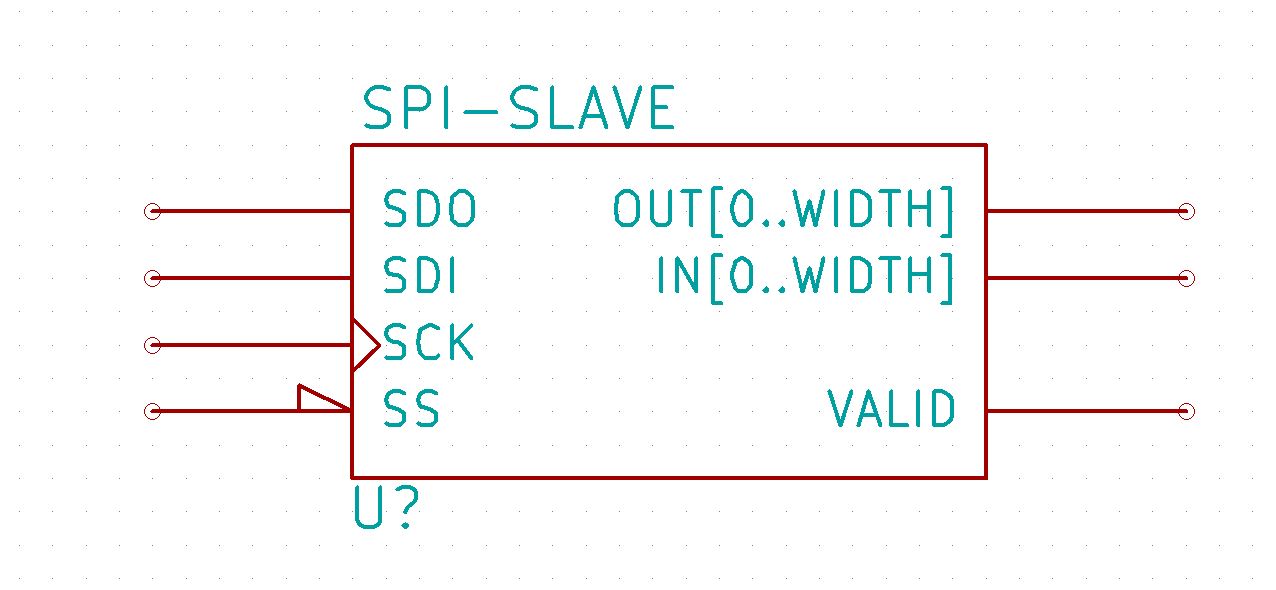
\includegraphics[width=0.9\textwidth]{img/SLAVE.png}
    \vspace{-1em}    
    \caption{Blockschaltbild des Slaves (ohne generische Parameter)}
    \label{fig:blockSlave}
\end{figure}
\newpage
Es existieren drei gemeinsame Leitungen, an denen jeder Teilnehmer angeschlossen ist:
\begin{itemize}
  \item [SDO] (englisch Serial Data Out) bzw. MISO oder SOMI (englisch Master in, Slave out)
  \item [SDI] (englisch Serial Data In) bzw. MOSI oder SIMO (englisch Master out, Slave in)
  \item [SCK] (englisch Serial Clock) bzw. SCLK, wird vom Master ausgegeben
  \item [OUT] ''Ausgaberegeister'' Parallele Ausgänge des Ausgangswort, je nach Wortbreite über
              \emph{generic} parametrisiert
  \item [IN]  ''Eingangsregeister'' Parallele Eingänge, je nach Wortbreite über
              \emph{generic} parametrisiert
  \item [VALID] Ausgang, welcher einen Impuls(halbe Periodenbreite) generiert wenn das Eingangswort
              gültig ist
\end{itemize}

Eine logisch-0 aktive Chip-Select-Leitungen, welche vom Master gesteuert wird. Diese Leitung wird je
nach Anwendung unterschiedlich mit Bezeichnungen wie SS, CS oder STE für Slave Select, Chip Select bzw.
Slave Transmit Enable bezeichnet, oft noch in Kombination mit einer Indexnummer zur Unterscheidung.
Es gibt auch spezielle Anwendungen, bei denen sich mehrere Slaves diese Leitung teilen. Viele
Einstellmöglichkeiten, beispielsweise mit welcher Taktflanke ausgegeben bzw. eingelesen wird,
Wortlänge, Übertragung MSB oder LSB zuerst.

Viele Einstellungsmöglichkeiten sind unter anderem deshalb erforderlich, weil sich die Spezifikation
für den SPI-Bus in vielen Dingen nicht konkret festlegt und deshalb verschiedene, zueinander
inkompatible Geräte existieren. So ist häufig für jeden angeschlossenen Schaltkreis eine eigene
Konfiguration des steuernden Mikrocontrollers (Master des SPI-Bus) erforderlich.

Es können theoretisch beliebig viele Teilnehmer an den Bus angeschlossen werden, wobei es immer
genau einen Master geben muss. Er ist derjenige, der das Clock-Signal an SCK erzeugt und festlegt,
mit welchem Slave er kommunizieren will. Das geschieht über die Leitung ''Slave Select''. Wird sie
gegen Masse gezogen, wird der jeweilige Slave aktiv, ''lauscht'' an MOSI und legt seine Daten im
Takt von SCK an MISO. Es wird somit ein Byte vom Master zum Slave und ein anderes Byte vom Slave zum
Master transportiert.

Ein Protokoll für die Datenübertragung wurde von Motorola zwar nicht festgelegt, doch haben sich in
der Praxis vier verschiedene Modi durchgesetzt. Diese werden durch die Parameter Clock Polarität
(CPOL) und Clock Phase (CPHA) festgelegt. Bei CPOL=0 ist der Clock Idle Low, bei CPOL=1 ist der
Clock Idle High. CPHA gibt nun an, bei der wievielten Flanke die Daten übernommen werden sollen. Bei
CPHA=0 werden sie bei der ersten Flanke übernommen, nachdem SS auf Low gezogen wurde, bei CPHA=1 bei
der zweiten. Somit werden die Daten bei CPOL=0 und CPHA=0 mit der ersten Flanke übernommen, die nur
eine High-Flanke sein kann. Bei CPHA=1 wäre es die zweite, also eine Low-Flanke. Bei CPOL=1 ist das
ganze folglich genau andersherum, bei CPHA=0 Low-Flanke und bei CPHA=1 High-Flanke.

Zu beachten ist noch, dass der Slave bei CPHA=0 seine Daten schon beim Runterziehen von SS an MISO
anlegt, damit der Master sie beim ersten Flankenwechsel übernehmen kann. Bei CPHA=1 werden die Daten
vom Slave erst beim ersten Flankenwechsel an MISO gelegt, damit sie beim zweiten Flankenwechsel vom
Master übernommen werden können. Der Master hingegen legt seine Daten immer zum gleichen Zeitpunkt
an, meist kurz nach der Low-Flanke von SCK.

Mit jeder Taktperiode wird ein Bit übertragen. Beim üblichen Bytetransfer sind also 8 Taktperioden
für eine vollständige Übertragung nötig. Es können auch mehrere Bytes hintereinander übertragen
werden, wobei nicht festgelegt ist, ob zwischen jedem Byte das SS-Signal kurz wieder auf High
gezogen werden muss. Eine Übertragung ist beendet, wenn das Slave-Select-Signal endgültig auf High
gesetzt wird.

\vspace{1em}
\begin{table}[h]
  \centering
  \begin{tabular}{| l || c | r |}
  \hline                        
  Mode & CPOL & CPHA \\
  \hline                        
  0 & 0 & 0 \\
  1 & 0 & 1 \\
  2 & 1 & 0 \\
  3 & 1 & 1 \\
  \hline  
  \end{tabular}
  \caption{Übersicht der verschiedenen Modi}
  \label{tab:modes}
\end{table}
\vspace{1em}
\begin{figure}[ht]
    \centering
    \vspace{-1em}
        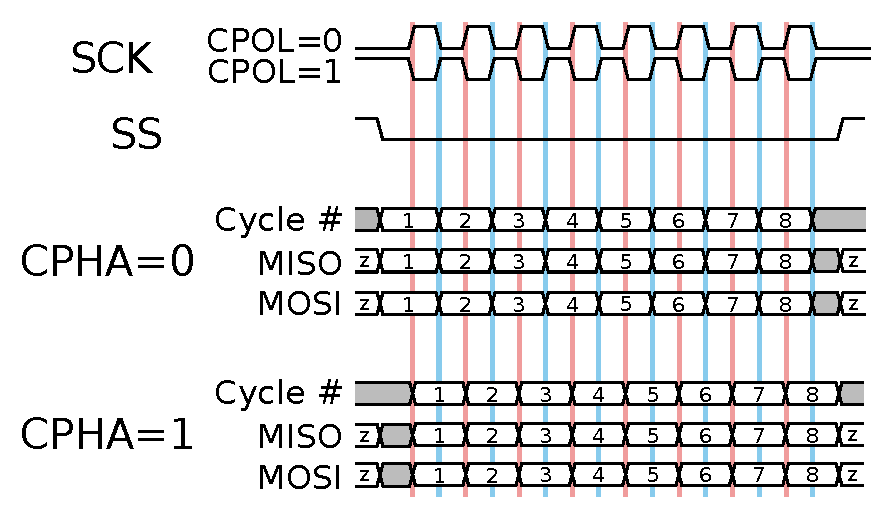
\includegraphics[width=0.9\textwidth]{img/SPItiming.pdf}
    \vspace{-1em}    
    \caption{Timing Diagramm zum SPI Protokoll}
    \label{fig:timing}
\end{figure}

\section{use-Cases}
Da eine genaue Wortbreite in der Spezifikation nicht vorgegeben ist, wird im folgendem von einem
8Bit breitem Datenwort ausgegangen.
Mögliche use-Cases sind:
\begin{itemize}
  \item Ein Datenwort empfangen/senden
  \item n Datenworte empfangen/senden
  \item fehlerhaftes Datenwort empfangen/senden
  \item n fehlerhafte Datenworte empfangen/senden
\end{itemize}

Diese sollten in allen vier Modi abgedeckt werden (siehe Tabelle \ref{tab:modes}).

\section{Lösungsansatz}
Nach dem Entwurf auf algorithmischer Ebene, wird das Modell mit der entsprechenden Testbench
verifiziert. Ist dieder Test erfolgreich, so ist ein Signalübergangsgraph zu entwerfen und aus Ihm
mit einer geeigneten Entwurfsmethode ein oder mehrere Automaten (Mealy/Moore/FSMD) abzuleiten.
Diese Realisierung ist wieder mit einer Testbench zu verifizieren (cycle accurate) und auf dem
DE2-Evaluationsboard zu implementieren.

	%% ...

	%% Beginn vom Anhang
	% \appendix
	%\pagenumbering{romanian}
	%\clearpage\setcounter{page}{2}

	%% Glossar
	% %\nomenclature{Begriff}{Erklärung des Begriffs}

\cleardoublepage% or \clearpage
\markboth{\nomname}{\nomname}

\printnomenclature
\addcontentsline{toc}{chapter}{Glossar und Abkürzungsverzeichnis}		

	%% Verzeichnisse
	\newpage
	\listoffigures
 	% \listoftables
	\lstlistoflistings

	%% Literaturverzeichnis
	% \newpage
	% \bibliographystyle{gerapali}
	% \bibliography{quellen}
	% \nocite{*}

	%% sonstiger Anhang:
	% \chapter{Anhang}
%-------------------------------------------------------------------------------------------------%
% - Quelltexte - %
%-------------------------------------------------------------------------------------------------%
\section{Quelltexte}
\lstset{language=C, inputencoding=utf8, literate={Ö}{{\"O}}1 {Ä}{{\"A}}1 {Ü}{{\"U}}1 {ß}{{\ss}}2
{ü}{{\"u}}1 {ä}{{\"a}}1 {ö}{{\"o}}1}

\lstset{label=code:headerglobal, caption=Globaler Header}
\lstinputlisting{code/global.h}
\lstset{label=code:sourceMain, caption=Main-Routine}
\lstinputlisting{code/main.c}

\end{document}
